\documentclass[tikz, border=5pt]{standalone}

\begin{document}

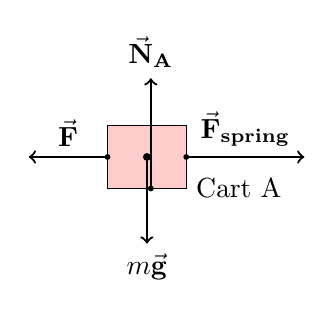
\begin{tikzpicture}

  % Cart A
  \draw[fill=red!20] (0,0) rectangle (1,0.8);
  \node [below, right] at (1,0) {Cart A};

  % Force F
  \draw[<-, thick] (-1,0.4) -- (0,0.4) node[midway, above] {\( \vec{\mathbf{F}} \)};
  \node[circle, fill, inner sep=0.75pt] at (0,0.4) {};

  % Spring Force
  \draw[->, thick] (1,0.4) -- (2.5,0.4) node[midway, above] {\( \mathbf{\vec{F}_{spring}} \)};
  \node[circle, fill, inner sep=0.75pt] at (1,0.4) {};

  % Normal reaction
  \draw[->, thick] (0.55,0) -- (0.55,1.4) node[above] {\( \mathbf{\vec{N}_A} \)};
  \node[circle, fill, inner sep=0.75pt] at (0.55,0) {};

  % Gravity
  \draw[->, thick] (0.5,0.4) -- (0.5,-0.7) node[below] {\( m\vec{\mathbf{g}} \)};
  \node[circle, fill, inner sep=1pt] at (0.5,0.4) {};

\end{tikzpicture}

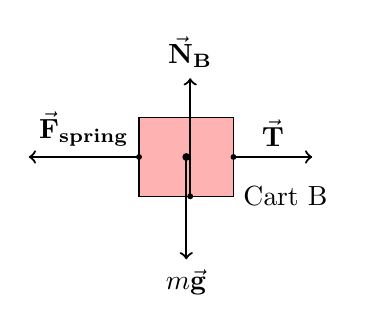
\begin{tikzpicture}

  % Cart B
  \draw[fill=red!30] (0,0) rectangle (1.2,1);
  \node [below, right] at (1.2,0) {Cart B};

  % Force T
  \draw[->, thick] (1.2,0.5) -- (2.2,0.5) node[midway, above] {\( \vec{\mathbf{T}} \)};
  \node[circle, fill, inner sep=0.75pt] at (0,0.5) {};

  % Spring Force
  \draw[<-, thick] (-1.4,0.5) -- (0,0.5) node[midway, above] {\( \mathbf{\vec{F}_{spring}} \)};
  \node[circle, fill, inner sep=0.75pt] at (1.2,0.5) {};

  % Normal reaction
  \draw[->, thick] (0.65,0) -- (0.65,1.5) node[above] {\( \mathbf{\vec{N}_B} \)};
  \node[circle, fill, inner sep=0.75pt] at (0.65,0) {};

  % Gravity
  \draw[->, thick] (0.6,0.5) -- (0.6,-0.8) node[below] {\( m\vec{\mathbf{g}} \)};
  \node[circle, fill, inner sep=1pt] at (0.6,0.5) {};

\end{tikzpicture}

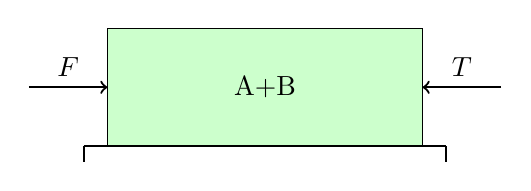
\begin{tikzpicture}

  % System
  \draw[fill=green!20] (0,0) rectangle (4,1.5);
  \node at (2,0.75) {A+B};

  % Force F
  \draw[->, thick] (-1,0.75) -- (0,0.75) node[midway, above] {$F$};

  % Force T
  \draw[->, thick] (5,0.75) -- (4,0.75) node[midway, above] {$T$};

  % Ground support
  \draw[thick] (-0.3,0) -- (4.3,0);
  \draw[thick] (-0.3,0) -- (-0.3,-0.2);
  \draw[thick] (4.3,0) -- (4.3,-0.2);

\end{tikzpicture}

\end{document}
